\section{Explications techniques des fonctions et composants}
	\subsection{Pont}
	\subsection{Terminal de recharge}
	\subsection{Terminal de paiement}
	\subsection{Serveur et base de données}
		Un serveur \og node \fg{} assisté du langage javascript a été utilisé pour construire les fonctionnalités \og backend \fg{} de notre projet. Le serveur est constitué de deux parties principales : un service d’api et un site web. 
		
		\subsubsection{API}
		Le service d’api est du format REST. Il permet d’accéder, d’ajouter, de modifier ou de retirer des ressources de la base de données. Chacune de ces opérations est sans état. L’avantage d’utiliser un api REST est que toutes les plateformes intégrant une fonctionnalité de requête HTTP et de sérialisation json peuvent facilement accéder à nos services de manière standardisée et agnostique aux détails d’implémentation de notre serveur. Voici une liste des services de notre api : %TODO Agnostique (2)
		%
		\begin{multicols}{3}
		\begin{itemize}
			\item Create Account
			\item Login Account
			\item Get Account
			\item List All Accounts
			\item Create Item
			\item Delete Item
			\item List Items
			\item Create Transaction
			\item List Transactions
		\end{itemize}
		\end{multicols}

		L’équipe a d’abord essayé d’utiliser les services ci-dessus avec le pont zigbee, cependant le micro-contrôleur du pont n’avait pas assez de mémoire pour sérialiser en JSON les informations reçues par ses n\oe{}uds, tel que mentionné précédemment. Cependant, les n\oe{}uds pouvaient le faire et le pont a donc été utilisé comme un relayeur des paquets JSON au serveur web. Toutefois, puisque le pont ne connaît pas le contenu des trames qu’il relaie, il ne peut envoyer ses requêtes qu’à un seul \og endpoint \fg{} de l’api REST. 

		Un \og endpoint \fg{} spécial nommé \og zigbee/bridge \fg{} a été créé pour désérialiser le JSON relayé par le pont zigbee et exécuter les actions nécessaires. Ce service comporte 4 fonctionnalités : 
		%
		\begin{itemize}
			\item Créer une transaction (débiter et créditer les bons comptes)
			\item Recevoir le montant restant sur un compte client
			\item Ajouter de l’argent à un compte
			\item Afficher le total pour un achat
		\end{itemize}

		
		\subsubsection{Site Web}
		Le site web est une interface qui permet aux marchands de voir leurs transactions effectuées, voir leurs produits, ajouter leurs produits et supprimer leurs produits. Les clients peuvent également accéder au site web pour voir leurs achats.
		
		\begin{figure}[p]
			\centering
			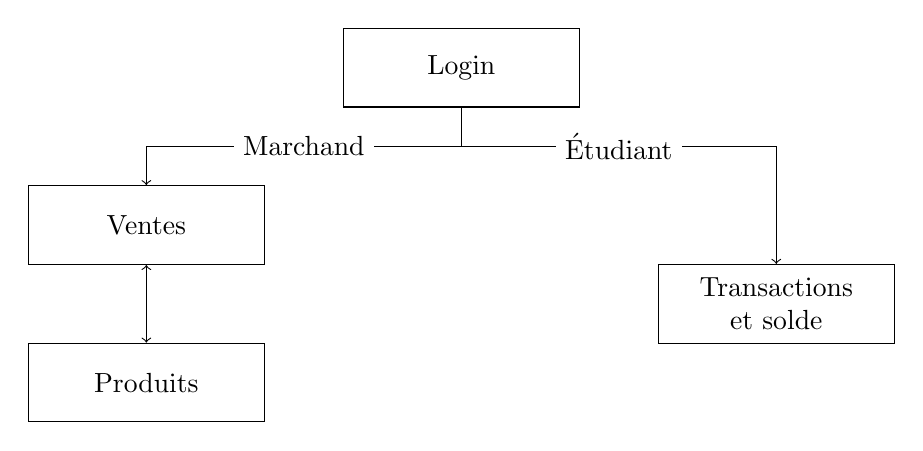
\begin{tikzpicture}[minimum height=1cm, minimum width=3cm, align=center]
	\node[draw] (prod) at (0,0) {Produits};
	\node[draw] (sales) at (0,2) {Ventes};
	\node[draw] (trans-solde) at (8,1) {Transactions \\ et solde};
	\node[draw] (login) at (4,4) {Login};
	%%%%%%%%%%%%%
	\draw[<->] (prod) -- (sales);
	\draw (login) -- (4,3);
	\draw (4,3) -- node[midway, fill=white, minimum size=0cm] {Marchand} (0,3);
	\draw (4,3) -- node[midway, fill=white, minimum size=0cm] {Étudiant} (8,3);
	\draw[->] (0,3) -- (sales);
	\draw[->] (8,3) -- (trans-solde);
\end{tikzpicture}
			\caption{Schéma des interactions avec le site web}
			\label{fig.schema}
		\end{figure}

		\begin{figure}[p]
			\fbox{\includegraphics[width=\textwidth]{Pictures/web/authentification}}
			\caption{Fenêtre d’authentification du site web (login)}
			\label{fig.auth}
		\end{figure}

		\begin{figure}[p]
			\fbox{\includegraphics[width=\textwidth]{Pictures/web/transSoldeEtudiant}}
			\caption{Transactions et solde d’un étudiant}
			\label{fig.transEtudiant}
		\end{figure}
		
		\begin{figure}[p]
			\fbox{\includegraphics[width=\textwidth]{Pictures/web/produitsMarchand}}
			\caption{Liste des produits d’un marchand}
			\label{fig.prodMarchands}
		\end{figure}

		\begin{figure}[p]
			\fbox{\includegraphics[width=\textwidth]{Pictures/web/ventesMarchand}}
			\caption{Ventes d’un marchand}
			\label{fig.ventesMarchands}
		\end{figure}

		Le site web a été créé sur le même serveur web que celui de l’api REST. Il utilise un modèle MVC. Il possède ses propres contrôleurs, routes et vues (\emph{views}), mais il partages ses modèles avec le service REST. Le \og rendering \fg{} de l’affichage se fait du côté serveur et des requêtes ajax sont utilisées pour rafraîchir les données automatiquement sans rafraîchissement de la page.
		
		\subsubsection{Postgres avec tables}
		Une base de données du format \emph{postgres} a été utilisée pour le projet, laquelle comporte 4 tables : 
		%
		\begin{itemize}
			\item Accounts
			\item Items
			\item Transactions
			\item LineItems
		\end{itemize}

		La table \og Accounts \fg{} comporte les comptes des clients et des marchands, leurs informations à propos de leur CIP, leurs cartes RFID, leur PIN et leur solde. La table \og Items \fg{}, fait la relation entre des items et un marchand qui les possède. La table \og LineItems \fg{} fait la relation entre des items, leur quantité et une transaction. La table \og Transactions \fg{} fait la relation entre un client et un marchand pour une transaction.

		Le plugin \og sequelize \fg{} a été utilisé pour faire nos modèles de la base de données en javascript et pour faire nos migrations de base de données ainsi que des \og seeds \fg{} pour la base de données.

		
		
		